% !TEX TS-program = pdflatex
% !TEX encoding = UTF-8 Unicode
%
% -----------------------------------------------------
% LaTeX-Vorlage
%
% LABREPORT v1
% von Markus Knösel frei nach KOMA-Script-Klassen
% -----------------------------------------------------
%
\documentclass[11pt,titlepage]{scrartcl}		% Schriftgröße festlegen, standard 10pt 
%
\usepackage[latin1]{inputenc}				% input encoding für vim/utf8/Umlaute
\usepackage[T1]{fontenc}
\usepackage{lmodern} 
%
% -----------------------------------------------------
\usepackage{geometry} 					% legt die Blattgröße und Randabstände fest
\geometry{a4paper}
\geometry{margin=3cm,top=2.5cm,bottom=2.5cm}
%
%
%
%
%
%
% -----------------------------------------------------
\usepackage{graphicx} 					% support the \includegraphics command and options
\usepackage[parfill]{parskip}				% Activate to begin paragraphs with an empty line rather than an indent
\usepackage{booktabs}					% for much better looking tables
%\usepackage{array}					% for better arrays (eg matrices) in maths
\usepackage{paralist}					% very flexible & customisable lists (eg. enumerate/itemize, etc.)
\usepackage{verbatim}					% adds environment for commenting out blocks of text & for better verbatim
\usepackage{subfig}					% make it possible to include more than one captioned figure/table in a single float
\usepackage{color}
\usepackage[german]{babel}
\usepackage{units}
\usepackage[onehalfspacing]{setspace}
\usepackage{amsmath,amsfonts,amssymb}
\usepackage{icomma,units}
\usepackage{enumerate}
\usepackage[margin=10pt,font=small,labelfont=bf,labelsep=endash]{caption}
\usepackage{chemmacros}
\usepackage{chemfig}
\usepackage{PSTricks}
\usepackage{epstopdf}
\usepackage[ngerman=ngerman-x-latest]{hyphsubst}
\usepackage{pgfplots}
\usepackage{pgfplotstable}
%
%
%
%
% ---------- HEADERS & FOOTERS ------------------------
\usepackage{fancyhdr} % This should be set AFTER setting up the page geometry
\pagestyle{fancy} % options: empty , plain , fancy
%\renewcommand{\headrulewidth}{0pt} % customise the layout...
\lhead{Markus Knösel}\chead{}\rhead{\textsc{Physikalische Chemie II}}
%\lfoot{}\cfoot{\thepage}\rfoot{}
%
%
%
%
% ---------- SECTION TITLE APPEARANCE -----------------
\usepackage{sectsty}
\definecolor{cyan}{RGB}{30,103,182}      % hellgruener Rahmen
\allsectionsfont{\mdseries\upshape\textcolor{cyan}} % (See the fntguide.pdf for font help)
%
%
%
%
% ---------- ToC (table of contents) APPEARANCE -------
\usepackage[nottoc,notlof,notlot]{tocbibind} % Put the bibliography in the ToC
\usepackage[titles,subfigure]{tocloft} % Alter the style of the Table of Contents
% \renewcommand{\cftsecfont}{\rmfamily\mdseries\upshape}
% \renewcommand{\cftsecpagefont}{\rmfamily\mdseries\upshape} % No bold!
%
%
%
%
% ---------- TITLEPAGE DETAILS ------------------------
\addtokomafont{subject}{\sc}
\setkomafont{title}{\normalfont}
	\subject{Amperometrische Fällungstitration von Bariumhydroxid mit Schwefelsäure}
	\title{Versuchsprotokoll}
	\subtitle{3812 - Praktikum Physikalische Chemie II}
	\author{\normalfont Markus Knösel \\ Matrikelnr. 23 94 86 }
	\date{durchgeführt am 14.11.14} % Activate to display a given date or no date (if empty),
\publishers{\normalsize \includegraphics[width=4cm]{unilogo} \\ Fachbereich IV \\ Abteilung für Chemie}
%
%
%
%
% ---------- DOCUMENT ---------------------------------
\begin{document}
	\maketitle
	\tableofcontents
	\newpage
%
%% \section*{\abstractname}
%% Blabla
%
\section{Theoretische Grundlagen}
In diesem Versuch soll durch amperometrische Titration die Konzentration einer gegebenen Bariumhydroxidlösung bestimmt werden. Dazu wird ein definiertes Volumen einer \ch{Ba(OH)2}Lösung unbekannter Konzentration mit Schwefelsäure bekannter Konzentration titriert und die Stromstärke bei einer angelegten Wechselspannung gemessen. Während der Titration fällt schwer lösliches Bariumsulfat aus:
\begin{reaction}
	Ba^2+ + SO4^2- -> BaSO4
\end{reaction}
Diese Fällungsreaktion macht sich in einem sinkendem Leitwert der Probelösung bemerkbar, es stehen weniger gelöste Ladungsträger zu Verfügung. Titriert man nun über den Äuivalenzpunkt hinaus, das heißt stehen keine \ch{Ba^2+}- und Hydroxidionen in Lösung mehr zur Verfügung, so steigt die Leitfähigkeit wieder an, da durch die Schwefelsäure nun vermehrt Ladungsträger eingebracht werden. Aus dem Leitfähigkeitsminimum läßt sich folglich die Konzentration der Bariumhydroxidlösung berechnen.
%
%
\section{Versuchsdurchführung}
\begin{figure}[h]
	\centering
	\scalebox{.6}{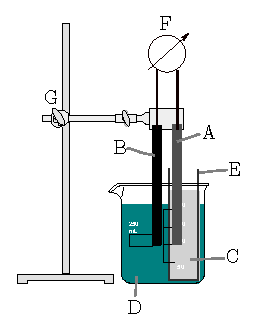
\includegraphics{aufbau.eps}}
	\caption{Versuchsaufbau}
	\label{fig:aufbau}
\end{figure}
%
\begin{singlespace}
	\small\underline{Geräte:}~Klemmen mit Muffen (A), Stativ (B), Bürette (C), Magnetrührer (D), Rührfisch (E), 2 Kupferelektroden (F), Wechselspannungsquelle (G), Amperemeter (H)\\[1ex]
	\underline{Chemikalien:}~gesättigte \ch{Ba(OH2)}-Lösung, Schwefelsäure ($c = 0,25 \unitfrac{mol}{l}$)\\[1ex]
\end{singlespace}
%
Die Versuchsapparatur wird gemäß Abbildung \ref{fig:aufbau} aufgebaut. In das Becherglas werden 50~ml einer gesättigten \ch{Ba(OH)2}-Lösung vorgelegt, in die Bürette wird bis zur 0-ml-Eichmarke Schwefelsäure eingefüllt. Vor der eigentlichen Titration wird die Bürette gründlich mit der Titrierlösung durchgespült, um Verunreinigungen und verdünnendes Wasser auszuspülen. Die Kupferelektroden werden so in die Lösung eingetaucht, daß genug Freiraum zum Eintropfen der Titrierlösung bleibt. An die Elektroden wird eine Wechselspannung von 2V angelegt, die Anfagsstromstärke wird notiert. Nun wird die Schwefelsäure in 1-ml-Schritten titriert, abgewartet bis die gemesene Stromstärke in etwa konstant bleibt und ihr Wert notiert. Die Messergebnisse finden sich in Tabelle \ref{tab:messwerte} im Anhang.
%
\subsection{Beobachtung}
%
Titriert man nun die vorliegende \ch{Ba(OH)2}-Lösung, so fällt sogleich ein weißer Niederschlsg von \ch{BaSO4} aus. Die Temperatur der Vorlage steigt merklich. Wie schon in Abschnitt 1 beschrieben, sinkt die elektrische Leitfähigkeit auf ein Minimum, um bei fortlaufender Titration wieder zu anzusteigen.
%
\section{Auswertung}
%
\begin{figure}[h]
	\centering
	\begin{tikzpicture}
	\begin{axis}[
			xlabel=$v_{(\ch{H2SO4})}$ in ml,
			ylabel=$I$ in mA,
			grid=major,
%			rotate=90,
%			anchor=origin, % Shift the axis so its origin is at (0,0)
%		rotate around={90:(current axis.origin)}, % Rotate around the origi
%		axis lines*=center,
	]
	\addplot table {daten.txt};
%	\addplot table[
%		x=v,
%	y={create col/linear regression}] %,
%		variance list={100}}]
%		{daten2.txt};
%	\addlegendentry{%
%       	$\pgfmathprintnumber{\pgfplotstableregressiona} \cdot x
%      	\pgfmathprintnumber[print sign]{\pgfplotstableregressionb}$ lin. Regression a}
%
	\addplot [black,domain=0:16, samples=200] {-12.34*x+201.2};
%	\addplot table[
%		x=v,
%	y={create col/linear regression}]
%		{daten3.txt};
%	\addlegendentry{%
%      	$\pgfmathprintnumber{\pgfplotstableregressiona} \cdot x
%      	\pgfmathprintnumber[print sign]{\pgfplotstableregressionb}$ lin. Regression b}
%
	\addplot [black,domain=14:23, samples=200] {21.64*x-302.22};
	\end{axis}
	\end{tikzpicture}
	\caption{Konzentrations-Stromstärke-Diagramm}
	\label{fig:graph}
\end{figure}
%
Während der Titration bis zur Vollständigen Fällung des \ch{BaSO4} sinkt die Leitfähigkeit pro ml hinzugefügter Schwefelsäure in kleinerem Maße, als die danach wieder ansteigt.\\
%
An die jeweiligen Äste des Leitfähigkeitstitrationsdiagrammes werden Ausgleichsgeraden angelegt. Die Regressionsfunktionen sind in Tabelle \ref{tab:linfit} im Anhang aufgeführt. Der Schnittpunkt dieser beiden Geraden - also das Volumen an hinzugefügter Schwefelsäure (hier $v$ = 14,8~ml) - liegt nun genau an dem Punkt, an dem das vorliegende \ch{Ba^2+} vollständig gefällt wurde. Ein Äquivalent Schwefelsäure (also ein \ch{SO4^2-}-Ion) fällt genau ein Äquivalent \ch{Ba^2+}. Die Konzentration der zu Beginn vorliegenden \ch{Ba^2+}-Ionen beträgt also
%
%\begin{reaction}
\begin{align*}
	c_{(\ch{Ba^{2+}})} &= \frac{v_{(\ch{H_2SO_4})} \cdot c_{(\ch{H2SO4})}}{v_{(\ch{Ba^{2+}})}} \\
    	&= 0,074~ \unitfrac{mol}{l}
\end{align*}
%
Geht man nun von einer reinen Bariumhydroxidlösung als Probelösung aus, so entspricht dies einer \ch{OH^-}-Konzentration von $c_{(\ch{OH^-})} = 2 \cdot c_{(\ch{Ba^{2+}})} = 0,148 \unitfrac{mol}{l}$. Das in diesem Versuch bestimmte Löslichkeitsprodukt von Bariumhydroxid beträgt folglich
%
\begin{align*}
	K_L &= c_{(\ch{Ba^{2+}})} \cdot {c_{(\ch{OH^-}})}^2 \\
	&= 4,0 \cdot 10^{-4} \unitfrac{mol^3}{l^3}
\end{align*}	
%
%\end{reaction}
%
%
\subsection{Systematische Fehlerbetrachung}
Die im Versuch bestimmte Konzentration an Bariumionen in Lösung weicht erheblich vom Literaturwert für die Konzentration an Ionen in gesättiger Lösung ab. \footnote{Aus dem Literaturwert für die Löslichkeit von \ch{BaSO4 * 8 \water} von 56~\unitfrac{g}{l} und einer Molmasse des Octahydrats von M=315,48 \unitfrac{mol}{l} ergibt sich eine \ch{Ba^2+}-Konzentration von 0,178~\unitfrac{mol}{l} bzw. ein Löslichkeitsprodukt $K_L$ von $5,6 \cdot 10^{-3}$ (\textsc{CRC}, B-74)} Eine Ursache hierfür wäre das Vermögen einer Bariumhydroxidlösung, aus der Luft Kohlenstoffdioxid aufzunehmen, sodaß sich unlösliches \ch{BaCO3} bildet und dadurch nicht mehr äquivalente Stoffmengen an Bariumionen und Hydroxidionen vorlägen. Zu Prüfen bleibt, was eine pH-Titration als Ergebnis der Konzentration an Hydroxidionen ergeben würde. Ebenfalls wäre eine Titerbestimmung der eingesetzten Schwefelsäure für die Fehlerbetrachtung sinnvoll.
Die Messungenauigkeiten der Volumenbestimmung der beiden Flüssigkeiten führen bei Fehlerfortpflanzung zu keinem signifikantem Fehler. \footnote{Die Fehlerfortpflanzung liefert eine Konzentrationsabweichung von lediglich $\Delta c = \pm 0,003~\unitfrac{mol}{l}$.}
%
%
%
\newpage
\section{Anhang}
%
\begin{table}[h]
	\centering
	\pgfplotstabletypesetfile[
		every head row/.style={before row=\toprule, after row=\midrule},
		every last row/.style={after row=\bottomrule},
		columns={v,I},
		columns/v/.style={
			column name= $v$ [ml]},
		columns/I/.style={
			column name= $I$ [mA]}
		]
		{daten.txt}	
	\caption{Messwerte}
	\label{tab:messwerte}
\end{table}
%
\begin{table}[h]
\centering
\begin{tabular}{lr}
	\toprule
	links: & $I = -12,34 \cdot v + 201,2$ \\
	\midrule
	rechts: & $I = 21,64 \cdot v -302,22$  \\
	\bottomrule
\end{tabular}
\caption{Regressionsfunktionen}
\label{tab:linfit}
\end{table}
%
\section{Literaturverzeichnis}
%
\textsc{Crc (1980-1981)}: \textit{Handbook of Chemistry and Physics}, 61st. Edition, CRC Press, Inc., Boca Raton, USA
%
\end{document}
